\chapter{Ordering in Inherent Structures}

The dynamic properties of the systems studied remains smooth and well behaved throughout the range simulated indicating that no phase transition took place over the range of temperatures studied. While the dynamics show no presence of a phase transition further study of the structure is necessary to rule out the possibility of ordering as a contributing factor in the behaviour of the dynamics. To remove the noise of vibrations from the structural analysis all the analysis in this chapter will be performed using inherent structures.


\section{The Lowest Energy Crystal Phases}

In the interests of developing more specific tools for detecting crystalline order, we need to know which crystal structures are likely to form. In most cases finding the crystal structure that is likely to form is a case of finding the lowest energy crystal structure. To find these lowest energy structures we need tools other than molecular dynamics since we chose systems to have crystallisation timescales at or beyond the limits of our simulations. To find a good approximation of the lowest energy structures we look to packing hard shapes, by modelling our molecules as hard discs we are able to use an isopointal algorithm to get a good approximation of the closest packed configurations. These closest packed configurations can be used as the starting configuration for our system to be equilibrated at a low temperature allowing the crystals to relax into their lowest energy state. \texttabref{crystal energies} shows the energy of the Lennard Jones systems that we are studying using the best packed isopointal structures for each wallpaper group as the starting configuration. Our Lennard-Jones system does not retain the constraints of the wallpaper group symmetry, however there are no significant deviations in the structure from that of the wallpaper group.

\begin{table}
    \sisetup{
        table-format = +3.4,
        table-omit-exponent,
        fixed-exponent =-4,
        parse-numbers=true,
        scientific-notation=true,
        round-mode=places,
        round-precision=3}
    \centering
    \begin{tabular}{ | l | S  S  S | }
        \hline
        {Crystal} & \multicolumn{3}{c|}{Energy per molecule (\num{e-4})} \\
            &\done & \dcon & \tri \\ \hline
        p2 & 0.00001376280055& {\cellcolor{blue!20}}0.0001527208398& {\cellcolor{blue!10}}-0.0003934685913\\
        p2mg & {\cellcolor{blue!20}}0.000005732595806& 0.0004479052484& -0.0003354198174\\
        p2gg & 0.00002632511042& 0.0001699363766& {\cellcolor{blue!20}}-0.000401823091\\
        pg & 0.00002824743917& 0.0002860863393& {\cellcolor{blue!10}}-0.0004000561542\\
        p3 & 0.00003468842645& 0.0002424453316& -0.0003292839541\\
        \hline
    \end{tabular}
    \caption{The energy per molecule for a variety of the best packing crystal structures. Both the \done and \dcon systems have an arrangement with significantly lower energy, p2mg and p2 respectively. While the \tri system has three arrangements with very similar energies, the p2, p2gg and pg wallpaper groups.}
    \label{tab:crystal energies}
\end{table}

With the \tri molecule having three crystal forms with similar energies, further analysis needs to be performed to elucidate the crystal structures that will form. Because the energies are so close together this moves from a search of structures, to the dynamics of crystal formation (full discussion on these systems in \textsecref{two phase}). For the \tri molecule in a system with a liquid-crystal boundary we observed a solid state rearrangement from the initial p2gg structure~\figref{tri rearr init} to a structure with bands of p2 crystal~\figref{tri rearr fine} telling us the p2 structure is more stable than the p2gg structure and the preferred of the three structures.

\begin{figure}
    \begin{subfigure}[t]{0.5\textwidth}
        \includegraphics[width=\textwidth]{{{Trimer-1.30-0.637556-1.00-120-p2gg-1-frame-0000000000}}}
        \caption{Initial p2gg structure of the \tri molecule. Note there are four layers of molecules.}
        \label{fig:tri rearr init}
    \end{subfigure}
    \begin{subfigure}[t]{0.5\textwidth}
        \includegraphics[width=\textwidth]{{{Trimer-1.30-0.637556-1.00-120-p2gg-1-frame-0320000000}}}
        \caption{In this configuration a number of the rows have switched orientations creating layers of p2 structure between the regions of p2gg structure.}
        \label{fig:tri rearr fine}
    \end{subfigure}
\caption{These configurations of the \tri molecule below the melting point show the solid-state phase transition that takes place.}
    \label{fig:tri two phase}
\end{figure}

Similarly as confirmation the three lowest energy crystal structures for the \done molecules were also simulated using a two phase system. Just like the \tri molecule the p2gg crystal of the \done molecule also a exhibited a solid state phase transition from the p2gg to the p2 crystal, both the p2gg and p2 crystals of the \done molecules had a lower melting point than the lowest energy \done crystal, p2mg. The high melting point of the p2mg crystal in the \done system compared to the other crystal structures confirms that the lowest energy p2mg structure is the most likely crystal to form. With the \dcon molecule only the p2 and p2gg structure were tested, these crystals had energies far below that of any other \dcon crystal structures. In this case the p2 structure had the higher melting point for the \dcon molecule again confirming the result we obtained from the energies.

\begin{table}
    \centering
    \begin{tabular}{| l l | S |}
        \hline
        Molecule & Crystal & {Melting Point} \\ \hline
        \multirow{3}{*}{\done} & p2 & 0.65 \\
                               & p2gg & 0.55 \\
                               & p2mg & 0.80 \\ \hline
        \multirow{2}{*}{\dcon} & p2 & 1.85 \\
                               & p2gg & 1.50 \\ \hline
    \end{tabular}
    \caption{Melting points of the crystal phases established from two phase systems}
    \label{tab:melting}
\end{table}

The lowest energy crystal structures we have determined for out molecules~\figref{crystals} consist of p2 and p2mg wallpaper groups. The p2 wallpaper group is the most heavily populated~\cite{plass:07,jennings:15} of the wallpaper groups, while the p2mg wallpaper group is rarely found in experimental systems~\cite{plass:07} . Both p2 and the p2mg structures exhibit an inversion center between pairs of molecules, a result that aligns with the crystal packing guidelines of~\textcite{torquato:12}.

Having worked out the crystal structures that are most likely to form for our molecules~\figref{crystals}, the properties of these crystal structures can be used to identify structures in the liquid phase that may indicate the presence of ordering.

\begin{figure}
    \centering
    \begin{subfigure}[t]{0.45\linewidth}
        \includegraphics[width=\textwidth]{{{Snowman-0.4-0.637556-1.00-p2mg-frame}}}
        \caption{The stable crystal phase of the \done molecule belongs to the p2mg wallpaper group.}
        \label{fig:crystal done}
    \end{subfigure}\hfill
    \begin{subfigure}[t]{0.45\linewidth}%
        \includegraphics[width=\textwidth]{{{Snowman-0.4-0.637556-1.637556-p2-frame}}}
        \caption{The stable crystal phase of the \dcon molecule belongs to the p2 wallpaper group.}
        \label{fig:crystal dcon}
    \end{subfigure}
    \begin{subfigure}{0.45\linewidth}
        \includegraphics[width=\textwidth]{{{Trimer-0.4-0.637556-1.00-120-p2-frame}}}
        \caption{The stable crystal phase of the \tri molecules belongs to the p2 wallpaper group.}
        \label{fig:crystal tri}
    \end{subfigure}
    \caption{The configurations of the stable crystal phases for each molecule. The molecules are coloured according to orientation. The unit cell is indicated by a black box and an inversion center is marked with a red dot.}
    \label{fig:crystals}
\end{figure}

\subsection{Order Parameters}

Taking what we know about the crystal structures we can develop order parameters which will aid in identifying regions of crystalline order. Along with crystalline order we also want to be able to identify other types of ordering including alignment of layers as would be found in a plastic-crystal. These more general forms of ordering form the basis of more specific techniques.

The radial distribution function $G(r)$ is one of the general techniques for detecting ordering in a simulated system. It is a distribution of the distances between the molecular centers of mass. The radial distribution of the \done molecule~\figref{done radial} shows an intense first shell peak, the immediate neighbours are at well defined distances. This order extends out to 12 units distance with \done molecule exhibiting broad peaks, indicating the presence of some weak medium-range ordering. The \dcon molecule~\figref{dcon radial} exhibits an intense first peak and some sharp secondary and second shell peaks. The intensity and sharpness of these peaks can be attributed to the interactions of the \dcon molecules as the concavity. The \dcon molecule has the largest concavity of the three molecules and when molecules are in the concavity they are highly constrained giving tight distributions of the center of mass~\figref{dcon radial part}. Unlike the sharp peaks of the \dcon molecule the \tri molecule~\figref{tri radial} has a series of three broad peaks in the first shell of neighbours, with order only extending to three broad peaks in the second shell. It is likely the concavities of the \tri molecule are much less selective than the concavities of the dimers.

\begin{figure}
    \centering
    \begin{subfigure}[t]{0.45\linewidth}
        \includegraphics[width=\linewidth]{{{Snowman-0.80-0.637556-1.0-radial}}}
        \caption{Radial distribution of \done molecule. The broad peaks out a distance of 12 indicate long range weak medium range ordering in the inherent structure.}
        \label{fig:done radial}
    \end{subfigure}\hfill
    \begin{subfigure}[t]{0.45\linewidth}
        \includegraphics[width=\linewidth]{{{Snowman-1.55-0.637556-1.637556-radial}}}
    \caption{Radial distribution of the \dcon molecule. The initial peaks are incredibly sharp showing strong short range ordering, however this order only extends to the second shell.}
        \label{fig:dcon radial}
    \end{subfigure}
    \begin{subfigure}{0.45\linewidth}
        \includegraphics[width=\linewidth]{{{Trimer-1.05-0.637556-1.00-120-radial}}}
        \caption{Radial distribution of the \tri molecule. All the peaks for this molecule are very broad, even in the first shell.}
        \label{fig:tri radial}
    \end{subfigure}
    \caption{Radial distribution function for each molecule showing a range of types of order.}
    \label{fig:radial distributions}
\end{figure}

\begin{figure}
    \centering
    \includegraphics[width=0.45\textwidth]{{{Snowman-1.55-0.637556-1.637556-radial2d_rel}}}
    \caption{The two dimensional radial distribution of the \dcon molecule in which the intensity of the peak is indicated by the amount of blue. The intense inner peaks (circled in red) show the distribution of the COM when the molecules interact via the concavity.}
    \label{fig:dcon radial2d_abs}
\end{figure}

Another measure of order is to look at the orientational distribution of the molecules. This provides an alternate look at the degree to which molecules are organising over large distances. The angular distribution looks at whether there are some directions which molecules are favouring, an indicator of long range ordering. None of the molecules~\figref{angular distributions} show a directional preference, a sign that there is no long range orientational ordering taking place.

\begin{figure}
    \centering
    \begin{subfigure}{0.45\linewidth}
        \includegraphics[width=\linewidth]{{{Snowman-0.80-0.637556-1.0-angular}}}
        \caption{The angular distribution of the \done molecule.}
        \label{fig:done angular}
    \end{subfigure}\hfill
    \begin{subfigure}{0.45\linewidth}
        \includegraphics[width=\linewidth]{{{Snowman-1.55-0.637556-1.637556-angular}}}
        \caption{The angular distribution of the \dcon molecule}
        \label{fig:dcon angular}
    \end{subfigure}
    \begin{subfigure}{0.45\linewidth}
        \includegraphics[width=\linewidth]{{{Trimer-1.05-0.637556-1.00-120-angular}}}
        \caption{The angular distribution of the \tri molecule.}
        \label{fig:tri angular}
    \end{subfigure}
    \caption{Angular distributions of the three molecules show no orientational ordering.}
    \label{fig:angular distributions}
\end{figure}

\subsection{Order in \dcon}

Both of the previous methods of describing order use properties of the molecule, the orientation and center of mass. In molecular systems these properties can fail to reflect the underlying structure. Consider the compact binary packing with a size ratio of 1:0.637556~\figref{compact}, an arrangement equivalent to packing the \dcon molecule without the allocation of bonds. The allocation of bonds can be performed randomly with no adjustment to the structure of the underlying particles. Two examples of assigning bonds; an ordered p2 structure~\figref{ordered frame}, and a randomly oriented structure~\figref{random frame} demonstrate the issues in identifying order with a random assignment of bonds. The orientational order of the p2 structure can easily be seen with diagonal banding of colours, corresponding to the two orientations present in the structure while the randomly assigned structure has molecules arranged with no orientational order, distributed between the eight possible molecular orientations. We can attempt to remove the noise of this orientational disorder by only plotting the centers of mass~(\textfigref{ordered com} and~\textfigref{random com}), however this gives a very similar result, the ordered structure exhibits distinctly crystalline behaviour with centers of mass aligning in rows while the random structure needs further analysis to be considered ordered.

\begin{figure}
    \centering
    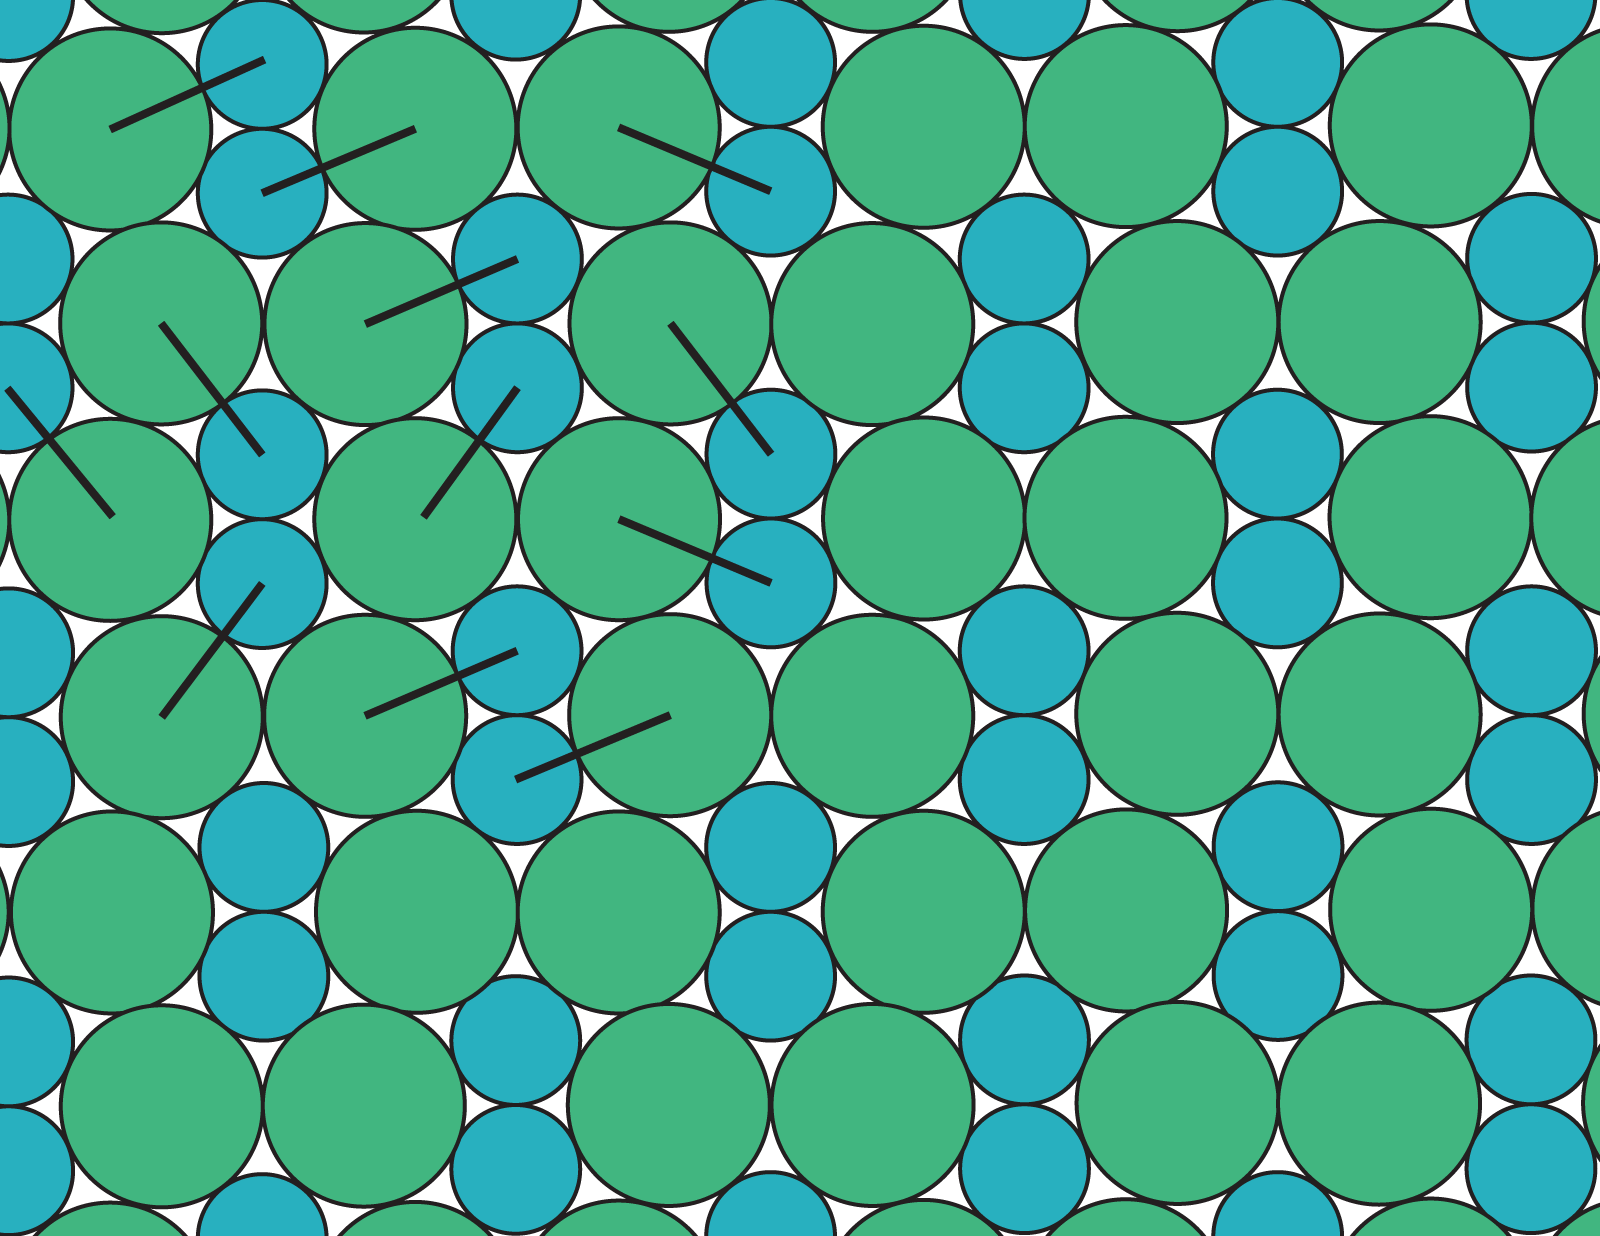
\includegraphics[width=0.5\textwidth]{compact}
    \caption{The compact packing of discs with ratio 1:0.637556. Assignment of bonds to this structure can be performed randomly (top left) with no alteration of the underlying structure.}
    \label{fig:compact}
\end{figure}

In the randomly oriented configuration the molecules are a construct placed on an ordered arrangement of particles. Since it is the particles define the order rather than the molecules, using an order parameter that is a measure of the ordering of the particles rather than the molecules is more appropriate for this molecule. If we define the \emph{particle radial distribution function} $G_p(r)$ in the same way as the radial distribution function, however instead of centers of mass we use the centers of density, the center of each disc. This particle radial distribution function translates better to experiments which look at the centers of density, each atom, rather than centers of mass. 

\begin{figure}
    \begin{subfigure}[t]{0.5\linewidth}
        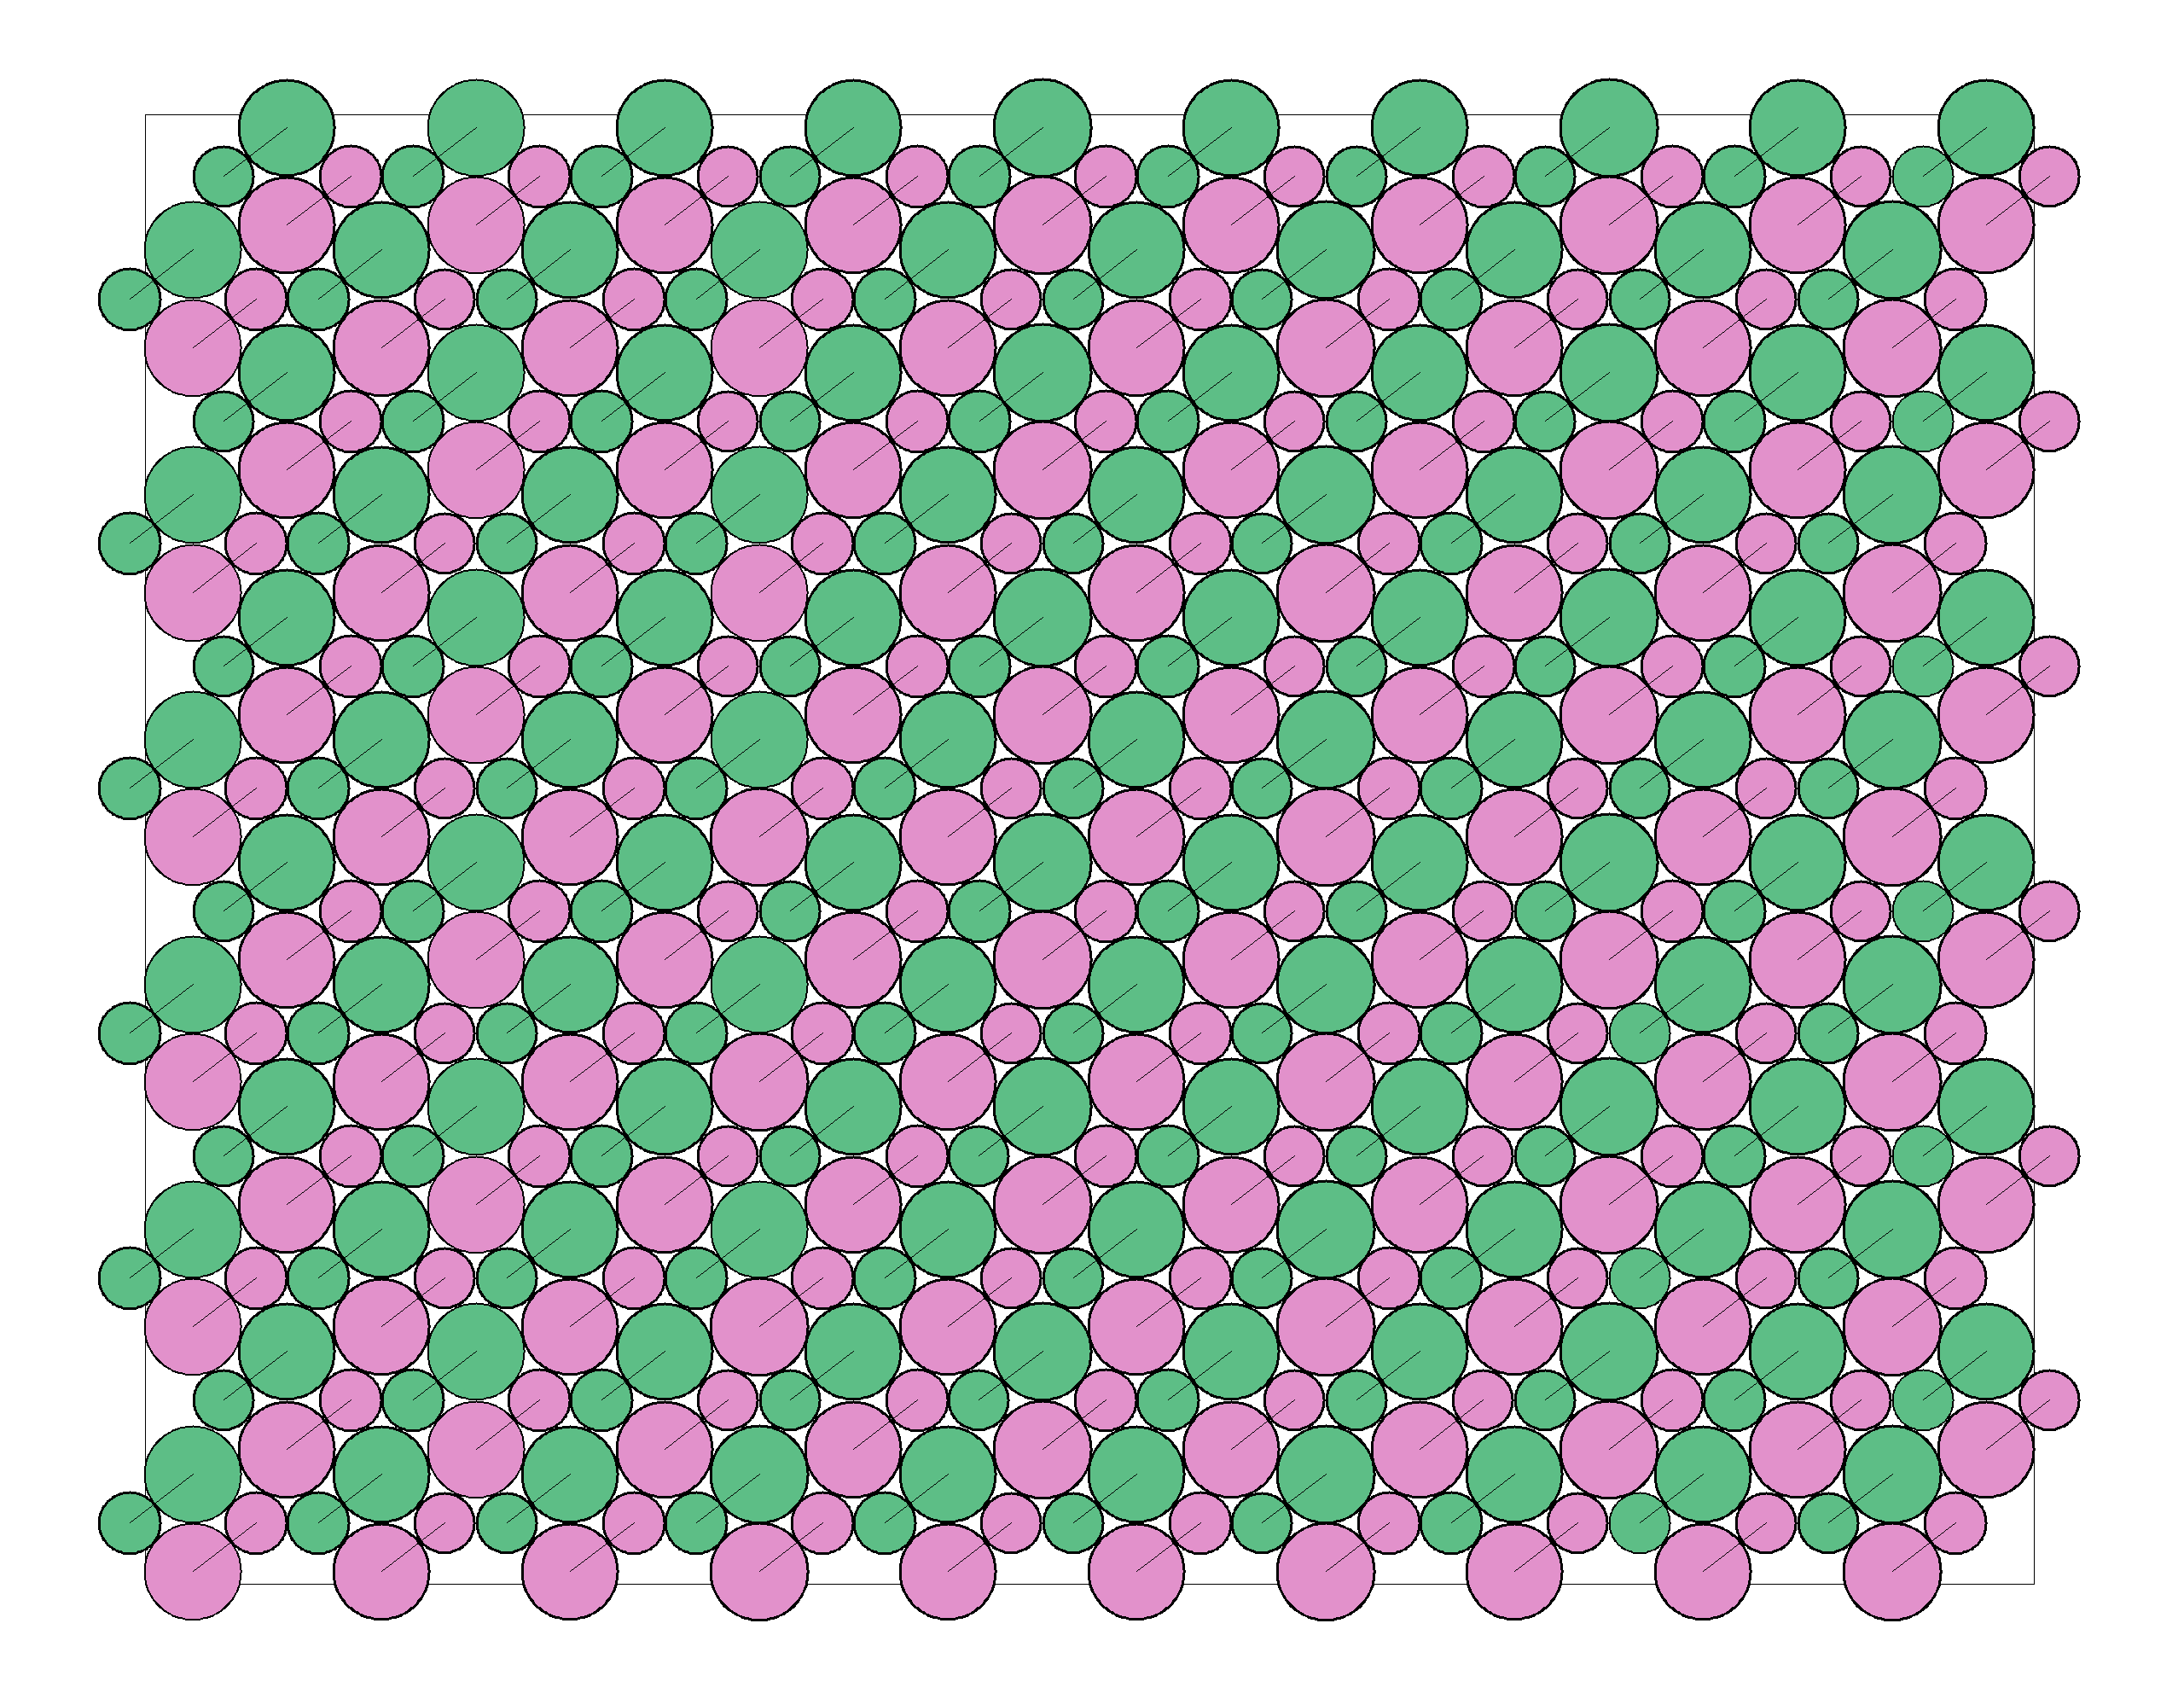
\includegraphics[width=\linewidth]{ordered-frame}
        \caption{A configuration of the \dcon molecule with p2 ordering.}
        \label{fig:ordered frame}
    \end{subfigure}
    \begin{subfigure}[t]{0.5\linewidth}
        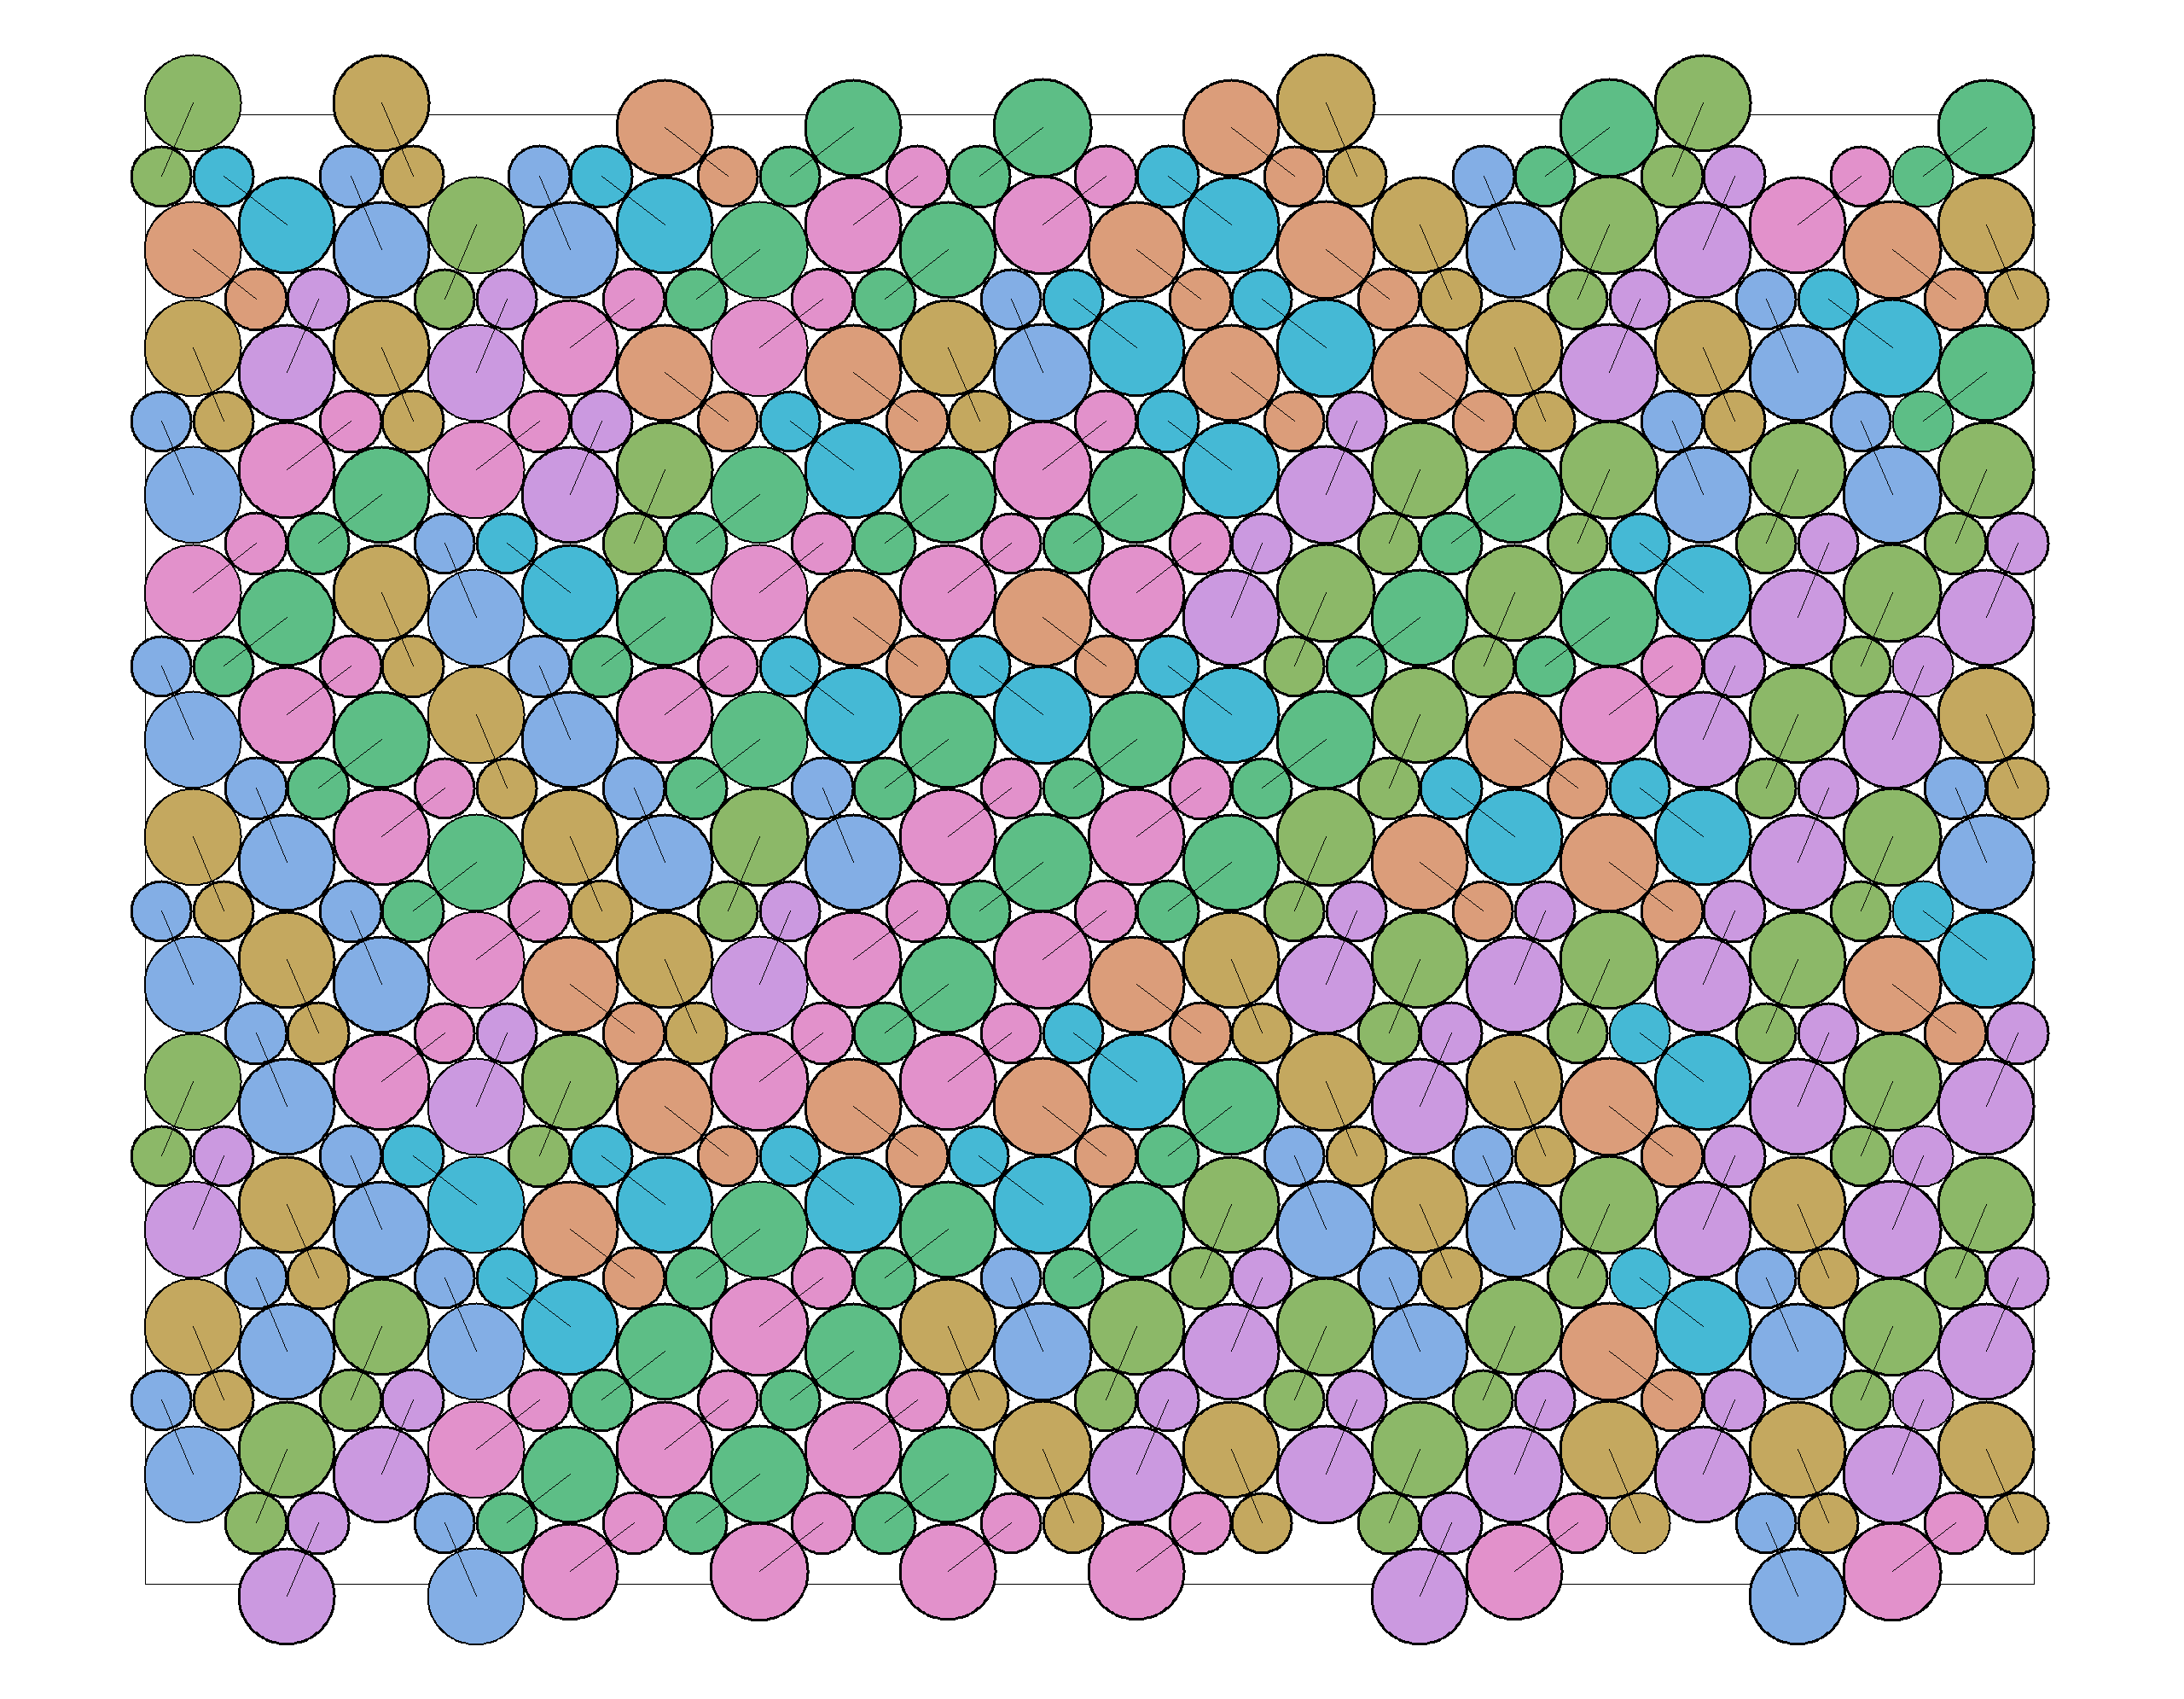
\includegraphics[width=\linewidth]{random-frame}
        \caption{A configuration of the \dcon molecule in which the bonds have been assigned randomly.}
        \label{fig:random frame}
    \end{subfigure}
    \begin{subfigure}[t]{0.5\linewidth}
        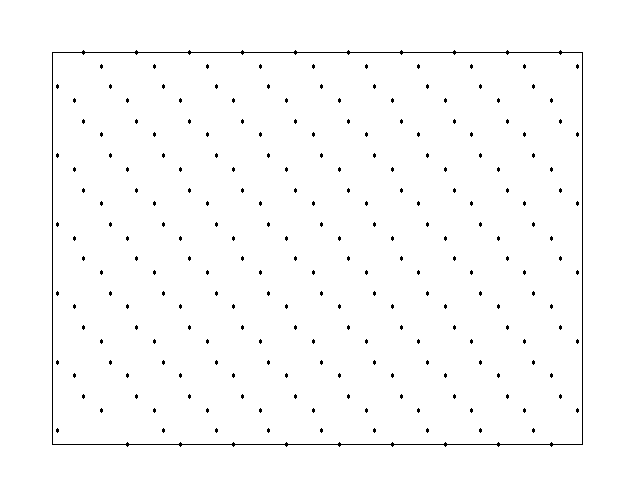
\includegraphics[width=\linewidth]{ordered-com}
        \caption{The COM of the \dcon molecule align when the configuration is crystalline.}
        \label{fig:ordered com}
    \end{subfigure}
    \begin{subfigure}[t]{0.5\linewidth}
        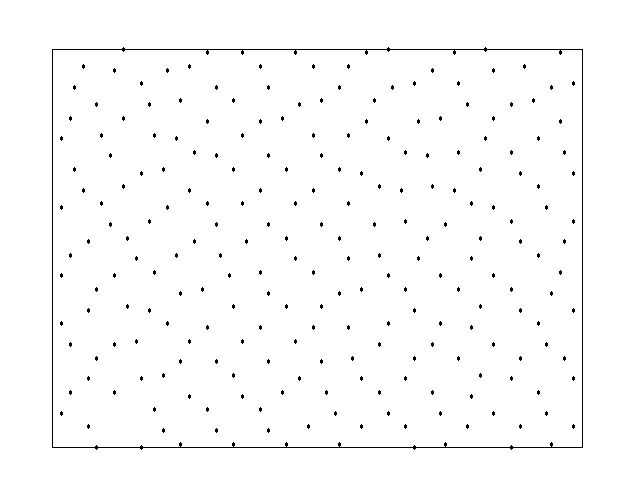
\includegraphics[width=\linewidth]{random-com}
        \caption{In the random configuration the COM of the \dcon molecule appear disordered.}
        \label{fig:random com}
    \end{subfigure}
    \begin{subfigure}[t]{0.5\linewidth}
        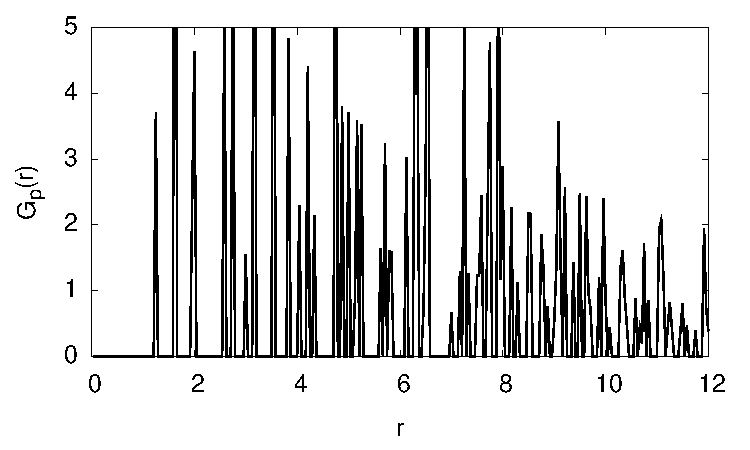
\includegraphics[width=\linewidth]{ordered-radial-part}
        \caption{The radial particle distribution function shows clear crystalline order in the sharp peaks.}
        \label{fig:ordered radial part}
    \end{subfigure}
    \begin{subfigure}[t]{0.5\linewidth}
        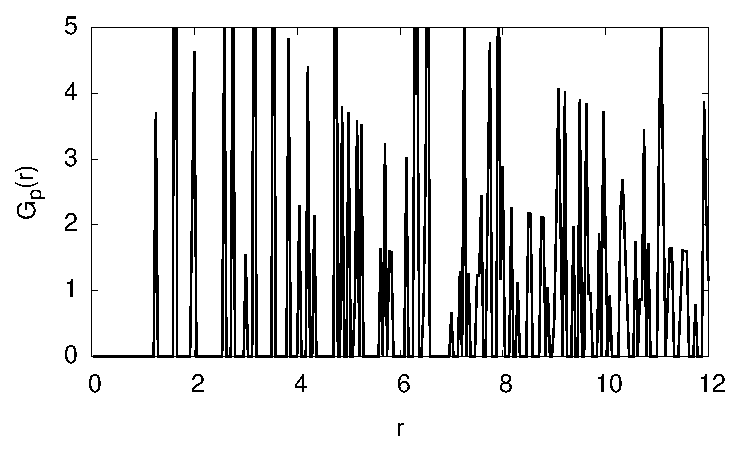
\includegraphics[width=\linewidth]{random-radial-part}
        \caption{The radial particle distribution function is essentially identical to the ordered structure.}
        \label{fig:random radial part}
    \end{subfigure}
    \caption{Comparison of the \dcon molecule with crystalline p2 ordering (left column) and random assignment of bonds (right column).}
    \label{fig:compact bonds}
\end{figure}


Using this particle radial distribution function we can look for order in the inherent structures of the molecules. The \dcon molecule~\figref{dcon radial part} shows medium range ordering which was not present on the radial distribution function~\figref{dcon radial}. The particle radial distribution function has also helped in reducing the number of secondary peaks with much sharper and higher intensity peaks. The \done molecule~\figref{done radial part} shows no medium range ordering unlike when using the radial distribution~\figref{done radial} which is an demonstrates the specificity of detecting order in these molecules. To get the best results order parameters need to be tailored to the particular molecule.

\begin{figure}
    \centering
    \begin{subfigure}[t]{0.45\linewidth}
        \includegraphics[width=\linewidth]{{{Snowman-0.80-0.637556-1.0-radial_part}}}
        \caption{Radial particle distribution function for the \done molecule.}
        \label{fig:done radial part}
    \end{subfigure}\hfill
    \begin{subfigure}[t]{0.45\linewidth}
        \includegraphics[width=\linewidth]{{{Snowman-1.55-0.637556-1.637556-radial_part}}}
        \caption{Radial particle distribution function for the \dcon molecule. This figure shows the presence of medium range ordering in the peaks extending out to a distance of 12.}
        \label{fig:dcon radial part}
    \end{subfigure}
    \begin{subfigure}{0.45\linewidth}
        \includegraphics[width=\linewidth]{{{Trimer-1.05-0.637556-1.00-120-radial_part}}}
        \caption{Radial particle distribution function for the \tri molecule.}
        \label{fig:tri radial part}
    \end{subfigure}
    \caption{Radial particle distribution for the three molecules.}
    \label{fig:radial part distributions}
\end{figure}

\section{Locality of Order}

We have the radial distribution functions and the orientational order parameters that inform us of order in the bulk. However these order parameters do not provide information on where the order is located, how many molecules are in these areas, whether there is a single crystal or is polycrystalline, and the size of any regions of order; a local order parameter can address all these problems. To take a local approach to order we have to find new order parameters that are capable of defining local order.

For the \done molecule we can define a local order parameter $O_\done$ based on the p2mg crystal structure as
\begin{equation}
    O_{\done} = \frac{1}{N_{\text{neigh}}}\sum_{i=1}^{N_\text{neigh}} (\vect{\hat e} \cdot \vect{\hat e_i})^2
\end{equation}
where $N_\text{neigh}$ is the number of neighbours, $\vect{\hat e}$ is the unit orientation vector of the molecule and $\vect{\hat e_i}$ is the unit orientation vector of each neighbour. Molecules that are above a cutoff of $0.8$ are considered to be crystalline while molecules below this cutoff are classed as amorphous. \textfigref{done inherent} demonstrates this order parameter using the inherent structure of the \done molecule studied throughout this chapter. There are many small regions of crystalline order while most of the configuration is amorphous.

In defining a local order parameter for the \dcon molecules we can use the particle approach that worked well for the global order parameter, however in this case we are looking at the local environment of each particle. In the p2 crystalline structure each small particle has one other small neighbour and four large neighbours, and each large particle has three small and three large neighbours. Molecules consisting of particles that have these specific neighbours are considered ordered.

The \tri molecule we are treating in the same way as the \done molecule, using the local orientational order of each molecule to assess the degree of ordering. For the \tri molecule the cutoff for this function was determined to be \num{0.7}, giving good differentiation between the crystal and liquid phases with an acceptable level of false positives and false negatives.

\begin{figure}
    \centering
    \begin{subfigure}[t]{0.45\linewidth}
        \includegraphics[width=\textwidth]{{{Snowman-0.80-0.637556-1.0-frame-0320000191}}}
        \caption{The configuration of \done shows regions of orientational order with layers of molecules arranged antiparallel to each other. These regions have different orientations indicating a series of nucleation events.}
        \label{fig:done inherent}
    \end{subfigure}\hfill
    \begin{subfigure}[t]{0.45\linewidth}
        \includegraphics[width=\textwidth]{{{Snowman-1.55-0.637556-1.637556-frame-0320000182}}}
        \caption{The \dcon molecule shows no sign of long range order. There are small clusters of particles exhibiting the orientationally disordered crystalline phase, however these only exhibit local interactions.}
        \label{fig:dcon inherent}
    \end{subfigure}
    \begin{subfigure}{0.45\linewidth}
        \includegraphics[width=\textwidth]{{{Trimer-1.00-0.637556-1.00-120-frame-0320000177}}}
        \caption{The \tri molecule shows no sign of ordering, a truly amorphous phase.}
        \label{fig:tri inherent}
    \end{subfigure}
    \caption{Final inherent structure configurations for each molecule, the colouring of the molecules representative of their orientations.}
    \label{fig:inherent structures frame}
\end{figure}

With these tools in detecting ordering in structures it is possible to detect the crystallisation of molecules.
